\subsection{Iterationen / Phasen}

Die zur Verfügung stehende Arbeitszeit wurde in sechs Iterationen zu jeweils
zwei Wochen und noch zwei Iterationen zu je einer Woche eingeteilt. Anhand der
bekannten Arbeitspaketen aus der Aufgabenstellung haben wir das Projekt in zwei
Phasen aufgeteilt. \\
In der ersten Phase haben wir uns den Pflichtteilen der Aufgabenstellung
angenommen. Die wesentlichen Ziele waren die Behebung der bereits bekannten Bugs
sowie die Implementation einer ersten Version des SWID Generators und der
entsprechenden Erweiterung der strongTNC App. \\
In der zweiten Phase konzentrierten wir uns in die Ausarbeitung des Konzeptes
strongTNC API, sowie architektonische Konzepte, die nicht Bestandteil der
Aufgabenstellung waren (siehe \autoref{analyse:soll-situation})

Das Ziel dieser Trennung war die Minimierung von Risiken, die erste Phase
erlaubte es Prototypen zu implementieren und die nötige Spezifikation zu
liefern, welche für die Integration in die strongSwan Infrastruktur nötig war.
Der detailierte Zeitplan ist im Anhang zu finden (\autoref{anhang:zeitplanung}).

\subsection{Zeiterfassung}

Während der gesamten Laufzeit der Arbeit haben wir für jeden Github Issue den
Zeitaufwand geschätzt und zusammen mit dem effektiven Aufwand in einem Google
Docs Spreadsheet festgehalten. Dies ermöglicht detaillierte Auswertungen der
benötigten Zeit sowie der Schätzungsgenauigkeit.

\subsubsection{Aufwand}

Der Aufwand pro Iteration stieg im Verlauf der Wochen stetig an (Abbildung
\ref{zeitanalyse:total}). In den ersten Iterationen war der Gesamtaufwand
geringer als später, weil eines unserer Teammitglieder unfallbedingt zwei Wochen
ausfiel. Dies ist auch gut in der Abbildung \ref{zeitanalyse:total-pro-person}
ersichtlich. \\
In der siebten Iteration stieg der Aufwand signifikant an, da wir die Feiertage
um Auffahrt nutzten um an dieser Arbeit weiterzuarbeiten. \\
Nach der sechsten Iteration war an der HSR Unterrichtsschluss, entsprechend
waren für die letzten zwei Iterationen mehr Zeit eingeplant. Die effektiv
geleistete Zeit überstieg diese jedoch noch stark.

Wie man in Abbildung \ref{zeitanalyse:tickets} sieht, korrelliert der geleistete
Aufwand korrelliert mit der Anzahl der geschlossenen Tickets pro Iteration. Mit
Abstand die meisten Tickets wurden in der siebten Iteration geschlossen. Dies
liegt einerseits am höheren Arbeitsaufwand, andererseits daran dass wir in
dieser Iteration mit intensivem Testen von strongTNC begonnen haben, was einige
neuen Bugs zu Tage brachte.

\subsubsection{Schätzungsgenauigkeit}

In der Abbildung \ref{zeitanalyse:abweichung} sieht, wurde die Zeitschätzung in
der ersten Hälfte der Arbeit immer besser, während sie sich in der zweiten Hälfte
wieder verschlechterte. \\
Die anfänglich hohe negative Abweichung liegt einerseits an unserer sehr
konservativen Schätzungsweise, andererseits daran dass aufgrund des Unfalls von
Danilo Bargen weniger Stunden geleistet wurden, als ursprünglich geschätzt
wurden. \\
In der Hälfte der Arbeit verbesserten sich die Schätzungen, in den letzten
Wochen verschlechterte sie sich jedoch wieder. Dies ist einerseits auf den
erhöhten Arbeitsaufwand zurückzuführen, andererseits auf den unterschätzten
Dokumentationsaufwand.

\begin{sidewaysfigure}
	\begin{minipage}[t]{0.45\textwidth}
		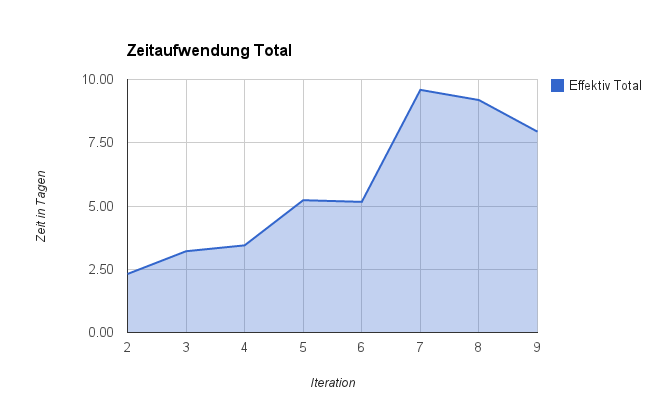
\includegraphics[width=\linewidth]{images/zeitplanung/chart_1}
		\caption{Zeitaufwendung Total}
		\label{zeitanalyse:total}
	\end{minipage}
	\hspace{\fill}
	\begin{minipage}[t]{0.45\textwidth}
		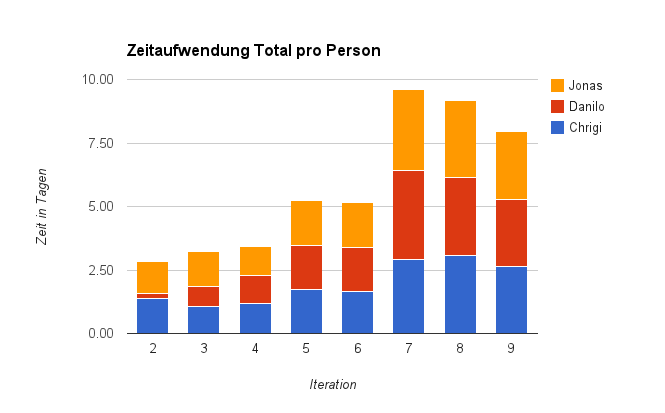
\includegraphics[width=\linewidth]{images/zeitplanung/chart_2}
		\caption{Zeitaufwendung Total pro Person}
		\label{zeitanalyse:total-pro-person}
	\end{minipage}

	\vspace{2cm}

	\begin{minipage}[t]{0.45\textwidth}
		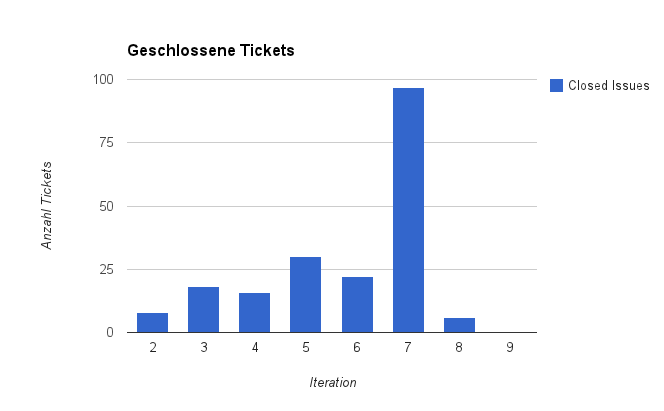
\includegraphics[width=\linewidth]{images/zeitplanung/chart_3}
		\caption{Geschlossene Tickets}
		\label{zeitanalyse:tickets}
	\end{minipage}
	\hspace{\fill}
	\begin{minipage}[t]{0.45\textwidth}
		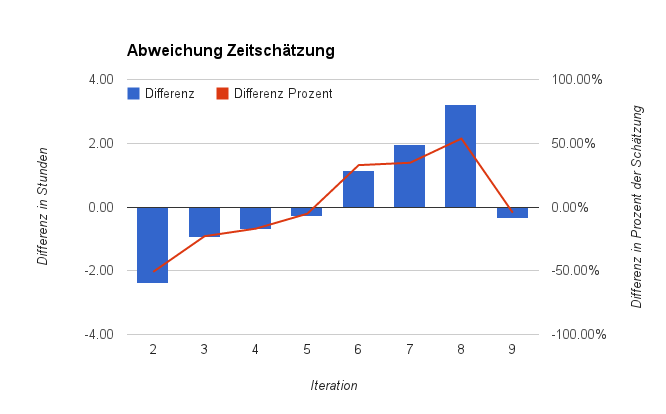
\includegraphics[width=\linewidth]{images/zeitplanung/chart_4}
		\caption{Abweichung Zeitschätzung}
		\label{zeitanalyse:abweichung}
	\end{minipage}

\end{sidewaysfigure}

\begin{sidewaysfigure}

	\begin{minipage}[t]{0.9\textwidth}
		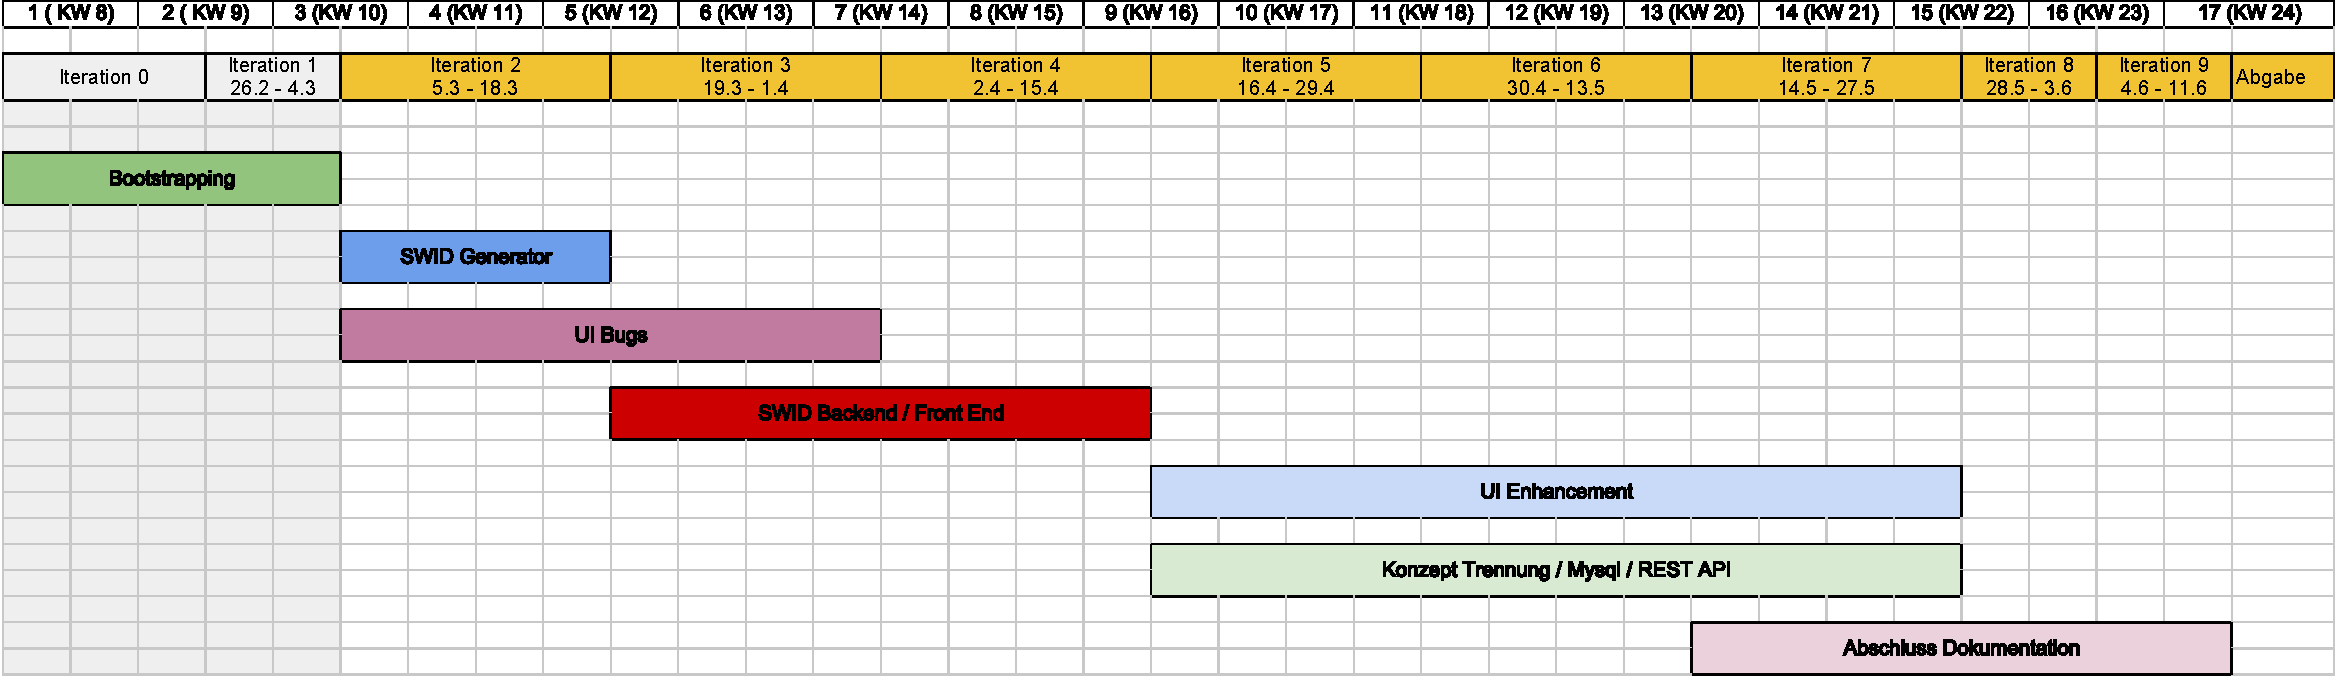
\includegraphics[width=\linewidth]{images/zeitplanung/iteration_1}
		\caption{Zeitplanung zu Beginn der Arbeit}
		\label{zeitanalyse:vorher}
	\end{minipage}

	\vspace{2cm}

	\begin{minipage}[t]{0.9\textwidth}
		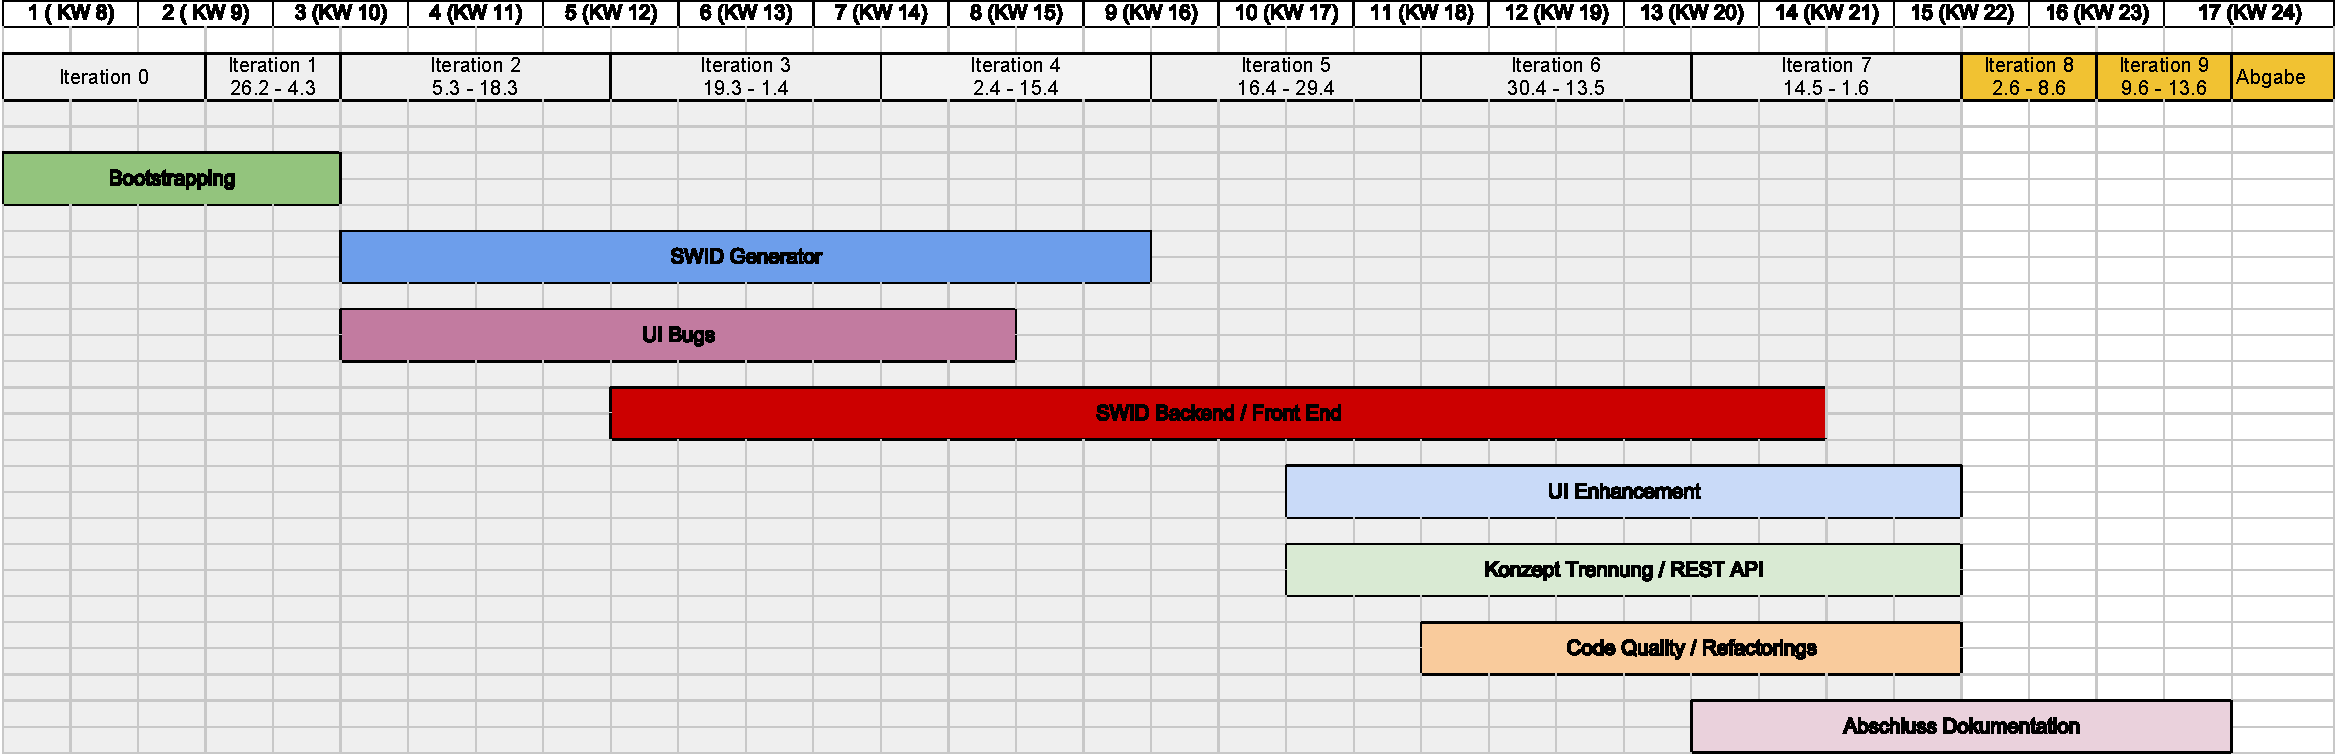
\includegraphics[width=\linewidth]{images/zeitplanung/iteration_8}
		\caption{Zeitplanung zum Schluss der Arbeit}
		\label{zeitanalyse:nachher}
	\end{minipage}

\end{sidewaysfigure}
